\documentclass[11pt]{article}
% =====================================================================
%  preamble.tex  --  SHARED PREAMBLE FOR CS-4031 COMPILER CONSTRUCTION
%  Fall 2026, FAST-NU Lahore
% =====================================================================

% ---------- Page geometry ----------
\usepackage[a4paper, margin=2.2cm, headsep=14pt, footskip=28pt]{geometry}

% ---------- Fonts / encoding ----------
\usepackage[utf8]{inputenc}
\usepackage[T1]{fontenc}

% ---------- Math ----------
\usepackage{amsmath, amssymb, amsthm}

% ---------- Colors ----------
\usepackage[table]{xcolor}
\definecolor{nuNavy}{HTML}{102A43}      % primary heading color
\definecolor{nuBlue}{HTML}{1B5FA8}      % accent / links
\definecolor{nuLight}{HTML}{EAF2FB}     % light panel background
\definecolor{dbGreen}{HTML}{1F7A4D}     % "Dragon Book / examinable" boxes
\definecolor{dbGreenBg}{HTML}{EAF7EF}
\definecolor{enrichGold}{HTML}{9A6A00}  % "enrichment / beyond DB" boxes
\definecolor{enrichGoldBg}{HTML}{FFF6E0}
\definecolor{examRed}{HTML}{B3261E}     % "exam focus" boxes
\definecolor{examRedBg}{HTML}{FCEBEA}
\definecolor{histPurple}{HTML}{5B3A8E}
\definecolor{histPurpleBg}{HTML}{F2EBFB}
\definecolor{takeawayTeal}{HTML}{0F6F6A}
\definecolor{takeawayTealBg}{HTML}{E7F6F5}
\definecolor{lightgray}{HTML}{F5F5F5}

% ---------- Headers / footers ----------
\usepackage{fancyhdr}
\pagestyle{fancy}
\fancyhf{}
\renewcommand{\headrulewidth}{0.6pt}
\renewcommand{\footrulewidth}{0.3pt}
\fancyhead[L]{\small\sffamily\color{nuNavy} CS-4031 Compiler Construction}
\fancyhead[R]{\small\sffamily\color{nuNavy} \rightmark}
\fancyfoot[L]{\small\sffamily\color{gray} FAST-NU Lahore, Fall 2026}
\fancyfoot[C]{\small\sffamily\color{gray} \thepage}
\fancyfoot[R]{\small\sffamily\color{gray} Notes by course staff}

% ---------- Section styling ----------
\usepackage{titlesec}
\titleformat{\section}
  {\normalfont\Large\bfseries\color{nuNavy}}
  {\thesection}{0.6em}{}
\titleformat{\subsection}
  {\normalfont\large\bfseries\color{nuBlue}}
  {\thesubsection}{0.6em}{}
\titlespacing*{\section}{0pt}{1.4em}{0.8em}
\titlespacing*{\subsection}{0pt}{1.1em}{0.5em}

% ---------- Lists, tables, misc ----------
\usepackage{enumitem}
\setlist{topsep=4pt, itemsep=2pt, parsep=0pt}
\usepackage{array, booktabs, tabularx, longtable, multirow}
\usepackage{graphicx}
\usepackage{tikz}
\usetikzlibrary{arrows.meta, positioning, shapes.geometric, fit, backgrounds, calc}
\usepackage{float}
\usepackage[colorlinks=true, linkcolor=nuBlue, citecolor=nuBlue, urlcolor=nuBlue]{hyperref}

% ---------- Table-of-contents number width ----------
% Default article.cls reserves just enough horizontal space in the TOC for a
% single-digit section number. Once any lecture grows past 9 top-level
% sections (as a merged/longer lecture can), two-digit numbers like "3.10"
% collide visually with the title text right after them ("3.10Extensions").
% tocloft lets us widen that reserved space once, here, so every lecture
% is protected regardless of how many sections it ends up with.
\usepackage{tocloft}
\setlength{\cftsecnumwidth}{2.8em}
\setlength{\cftsubsecnumwidth}{3.4em}
\renewcommand{\theHsection}{L\thelecnum.\arabic{section}}
\renewcommand{\theHsubsection}{L\thelecnum.\arabic{section}.\arabic{subsection}}
\renewcommand{\theHsubsubsection}{L\thelecnum.\arabic{section}.\arabic{subsection}.\arabic{subsubsection}}

% ---------- Cross-reference machinery (no hard-coded section/lecture numbers) ----------
% Every lecture resets \setcounter{section}{0} at its own top (see \lecturemeta / the
% \setcounter{section}{0} call in each lecture file), so within a single lecture, sections
% would normally print as a bare "1", "2", "3", ... -- indistinguishable at a glance from the
% *next* lecture's own "1", "2", "3", ... once everything is stitched into one combined PDF.
% Prefixing the *displayed* section number with the lecture number fixes this without touching
% any individual lecture file: "3.2" unambiguously means "Lecture 3, Section 2" everywhere,
% including in the combined table of contents.
\renewcommand{\thesection}{\thelecnum.\arabic{section}}

% \Sref{<label>} is the standard way to refer to a section from prose, in place of typing a
% literal number. Pair every \section/\subsection that is ever referred to elsewhere with a
% \label{sec:...} right after it, then write \Sref{sec:...} wherever the old text would have
% hard-coded "\S2.4" or similar. If the numbering ever shifts (a new section inserted, content
% reordered), every \Sref pointing at that label updates automatically on the next compile.
\newcommand{\Sref}[1]{\S\ref{#1}}


% ---------- Box framework (tcolorbox) ----------
\usepackage[most]{tcolorbox}
\tcbuselibrary{skins, breakable}

\newtcolorbox{lecbox}[3]{
  breakable, enhanced, sharp corners=downhill,
  colback=#2, colframe=#1,
  boxrule=0.6pt, left=6pt, right=6pt, top=4pt, bottom=4pt,
  fonttitle=\bfseries\sffamily, coltitle=white,
  colbacktitle=#1,
  title={#3},
  attach boxed title to top left={yshift=-0.3mm, xshift=2mm},
  boxed title style={sharp corners, colframe=#1, boxrule=0pt},
  top=8mm
}

\newenvironment{coreidea}[1][Core Idea (Dragon Book)]
  {\begin{lecbox}{dbGreen}{dbGreenBg}{#1}}
  {\end{lecbox}}

\newenvironment{examfocus}[1][Exam Focus]
  {\begin{lecbox}{examRed}{examRedBg}{#1}}
  {\end{lecbox}}

\newenvironment{enrichment}[1][Beyond the Dragon Book -- Enrichment]
  {\begin{lecbox}{enrichGold}{enrichGoldBg}{#1}}
  {\end{lecbox}}

\newenvironment{historynote}[1][A Bit of History]
  {\begin{lecbox}{histPurple}{histPurpleBg}{#1}}
  {\end{lecbox}}

\newenvironment{takeaways}[1][Key Takeaways]
  {\begin{lecbox}{takeawayTeal}{takeawayTealBg}{#1}}
  {\end{lecbox}}

\newtcolorbox{defbox}[1]{
  breakable, enhanced, colback=nuLight, colframe=nuBlue,
  boxrule=0.5pt, left=6pt, right=6pt, top=3pt, bottom=3pt,
  fonttitle=\bfseries, coltitle=nuNavy,
  title={Definition: #1}
}
\newtcolorbox{examplebox}[1]{
  breakable, enhanced, colback=white, colframe=gray!60,
  boxrule=0.5pt, left=6pt, right=6pt, top=3pt, bottom=3pt,
  fonttitle=\bfseries, coltitle=black,
  title={Example: #1}
}

% ---------- Lecture metadata machinery ----------
\newcommand{\thelecnum}{}
\newcommand{\lecshorttitle}{}
\newcommand{\lecclo}{}
\newcommand{\lecdbrefs}{}
\newcommand{\lecotherrefs}{}
\newcommand{\lecfulltitle}{}

\newcommand{\lecturemeta}[5]{%
  \global\renewcommand{\thelecnum}{#1}%
  \global\renewcommand{\lecfulltitle}{#2}%
  \global\renewcommand{\lecclo}{#3}%
  \global\renewcommand{\lecdbrefs}{#4}%
  \global\renewcommand{\lecotherrefs}{#5}%
}
\newcommand{\lecshort}[1]{%
  \global\renewcommand{\lecshorttitle}{#1}%
  \markright{Lecture \thelecnum\ --- #1}%
}

% ---------- Per-lecture \label and table-of-contents entry ----------
% \lecturelabel defines \label{lec:<N>} so other lectures can write "Lecture~\ref{lec:5}"
% instead of a hard-coded "Lecture 5" that silently goes stale if lectures are ever
% renumbered or reordered. \label normally captures whatever \thesection/\thechapter/etc.
% last set as \@currentlabel; since a bare lecture title isn't a sectioning command, we set
% \@currentlabel to \thelecnum ourselves first, so \ref{lec:<N>} prints just the number.
% \makeatletter/\makeatother are required here: \@currentlabel contains "@", which is not a
% letter by default in a plain \input file like this one (only inside .cls/.sty loading does
% LaTeX make that automatic) -- without this, "\@currentlabel" tokenizes as the unrelated
% control-symbol "\@" followed by the literal word "currentlabel", silently missing the
% kernel's real \@currentlabel entirely and leaving every \ref{lec:...} blank.
\makeatletter
\newcommand{\lecturelabel}{%
  \global\edef\@currentlabel{\thelecnum}%
  \label{lec:\thelecnum}%
}
\makeatother

% \lecturetocentry inserts one bold, page-level line into the *combined* table of contents
% for this lecture, at the same outline depth LaTeX normally reserves for \part -- one level
% above \section. This is what turns the combined TOC from a flat, ambiguous run of
% "1, 2, 3, 1, 2, 3, 4, ..." into a clearly hierarchical "Lecture 1: <title> / 1.1 ... / 1.2
% ... // Lecture 2: <title> / 2.1 ... / ...". It only affects the TOC listing -- it does not
% print a page break or heading in the body, since \makelecturetitle already provides that.
\newcommand{\lecturetocentry}{%
  \phantomsection
  \addcontentsline{toc}{part}{Lecture \thelecnum: \lecshorttitle}%
}

\newcommand{\makelecturetitle}{%
  \lecturelabel
  \lecturetocentry
  \begin{center}
    {\small\sffamily\color{gray} THE NATIONAL UNIVERSITY OF COMPUTER AND EMERGING SCIENCES, LAHORE}\\[2pt]
    {\small\sffamily\color{gray} CS-4031 Compiler Construction --- Fall 2026}\\[10pt]
    {\Huge\bfseries\color{nuNavy} Lecture \thelecnum}\\[4pt]
    {\LARGE\bfseries\color{nuBlue} \lecfulltitle}
  \end{center}
  \vspace{6pt}
  \noindent
  \begin{tcolorbox}[breakable, enhanced, colback=nuLight, colframe=nuNavy,
      boxrule=0.6pt, left=8pt, right=8pt, top=4pt, bottom=4pt]
    \small
    \begin{tabularx}{\textwidth}{@{}l X@{}}
      \textbf{CLO(s) covered:} & \lecclo \\
      \textbf{Dragon Book [DB]:} & \lecdbrefs \\
      \textbf{Other references:} & \lecotherrefs \\
    \end{tabularx}
  \end{tcolorbox}
  \vspace{4pt}
}

\newcommand{\beyonddb}{\textcolor{enrichGold}{\small\textbf{[beyond DB]}}\ }
\newcommand{\dbtag}{\textcolor{dbGreen}{\small\textbf{[DB]}}\ }

% ---------- Bibliography convention ----------
% Each lecture file ends its own "References for This Lecture" section with a
% \begin{thebibliography}{99} ... \end{thebibliography} block (no external .bib file or
% bibtex pass needed -- \cite{} resolves against \bibitem entries in the same document via
% the normal two-pass pdflatex + .aux mechanism already used for every other cross-reference
% here). A lecture only lists the \bibitem entries it actually \cite{}s.
%
% To keep citation keys consistent as more lectures are added, reuse these canonical keys
% (and the same canonical \bibitem text) rather than inventing new ones for the same source:
%   db        Aho, Lam, Sethi, Ullman -- Compilers: Principles, Techniques, and Tools (2nd ed.)
%   et        Cooper & Torczon -- Engineering a Compiler (2nd ed.)
%   ap        Appel -- Modern Compiler Implementation in C/Java/ML
%   pp        Scott -- Programming Language Pragmatics
%   mu        Muchnick -- Advanced Compiler Design and Implementation
%   an        Parr -- The Definitive ANTLR 4 Reference
%   gr        Gries -- Compilers: A Survey
%   llvmlangref   LLVM Language Reference Manual
%   llvmka        "My First Language Frontend with LLVM" (Kaleidoscope Tutorial)
%   antlrsite     ANTLR4 project site
%   tssite        Tree-sitter site
%   mlir          Lattner et al., "MLIR: A Compiler Infrastructure for the End of Moore's Law"
%   mlirdocs      The MLIR Project, official documentation
% A "Citation ... multiply defined" warning in the combined full-course-notes.pdf build (when
% two lectures both cite, say, \bibitem[DB]{db}) is expected and harmless: each lecture's own
% thebibliography block is independent, the canonical text is identical everywhere it is
% reused, and the explicit [DB]-style label (not an auto-generated number) is what actually
% gets printed, so it renders identically regardless of which instance "wins" in the aux file.


\lecturemeta{2}
  {Structure of a Compiler: Phases Overview; Front-/Middle-/Back-End; Preprocessor, Assembler, Linker, Loader}
  {CLO 1}
  {\S1.2 (The Structure of a Compiler), \S2.1--\S2.8 (overview of a syntax-directed translator's stages)}
  {[PP] Programming Language Pragmatics \S1.5, \S1.6}
\lecshort{Structure of a Compiler}

\begin{document}
\makelecturetitle

\begin{coreidea}[Lecture Roadmap]
\begin{enumerate}
  \item The classical phase pipeline of a compiler (DB Fig.\,1.6): what each phase consumes and
  produces.
  \item The two cross-cutting components every phase touches: the \textbf{symbol table} and
  \textbf{error handling}.
  \item Grouping the phases into \textbf{front-end / middle-end / back-end}, and why that
  grouping is an engineering decision, not just a diagram convenience.
  \item The compiler's \textbf{neighbors} in the full toolchain: preprocessor, assembler,
  linker, and loader --- what runs before and after the compiler proper.
\end{enumerate}
Today is still ``the outside view.'' From Lecture 3 onward we go phase-by-phase in depth,
starting with lexical analysis.
\end{coreidea}

\section{The Phase Pipeline of a Compiler}

\dbtag DB organizes a compiler as a pipeline of phases, each of which takes the output of the
previous phase as input, checks it, and produces a new representation of the program one step
closer to executable code.

\begin{center}
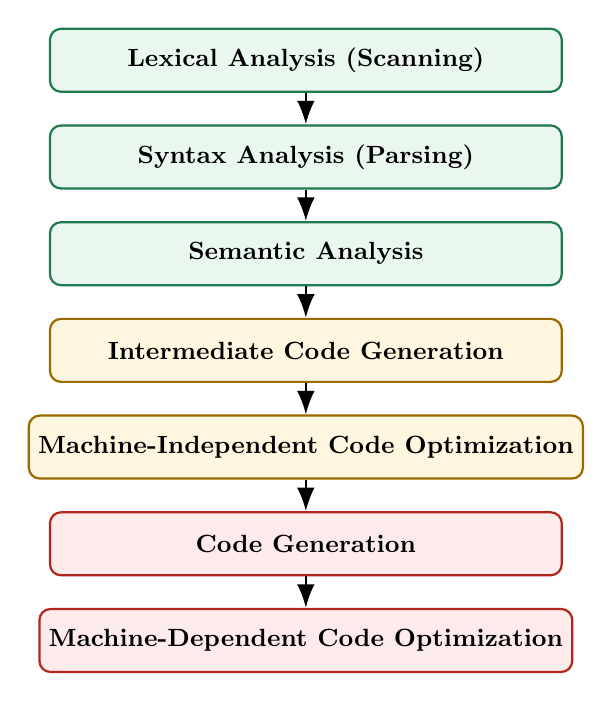
\begin{tikzpicture}[
  ph/.style={draw, thick, rounded corners, minimum height=0.8cm, minimum width=6.5cm, align=center, font=\bfseries\small},
  fe/.style={ph, fill=dbGreenBg, draw=dbGreen},
  mid/.style={ph, fill=enrichGoldBg, draw=enrichGold},
  be/.style={ph, fill=examRedBg, draw=examRed},
  node distance=0.4cm
]
  \node[fe] (lex) {Lexical Analysis (Scanning)};
  \node[fe, below=of lex] (syn) {Syntax Analysis (Parsing)};
  \node[fe, below=of syn] (sem) {Semantic Analysis};
  \node[mid, below=of sem] (icg) {Intermediate Code Generation};
  \node[mid, below=of icg] (opt) {Machine-Independent Code Optimization};
  \node[be, below=of opt] (cg) {Code Generation};
  \node[be, below=of cg] (mopt) {Machine-Dependent Code Optimization};

  \foreach \a/\b in {lex/syn, syn/sem, sem/icg, icg/opt, opt/cg, cg/mopt}
    \draw[-{Latex[length=3mm]}, thick] (\a) -- (\b);
\end{tikzpicture}
\end{center}

\begin{center}
\renewcommand{\arraystretch}{1.3}
\begin{tabularx}{\textwidth}{@{}l l X@{}}
\toprule
\textbf{Phase} & \textbf{Input} & \textbf{Output} \\
\midrule
Lexical Analysis & Raw character stream & Stream of \textbf{tokens} (e.g.\ \texttt{ID}, \texttt{NUM}, \texttt{+}) \\
Syntax Analysis & Token stream & \textbf{Syntax tree} (or parse tree) capturing grammatical structure \\
Semantic Analysis & Syntax tree & Annotated (``decorated'') tree: types checked, scopes resolved \\
Intermediate Code Gen. & Annotated tree & Machine-independent \textbf{IR}, e.g.\ three-address code \\
Code Optimization & IR & Improved, semantically-equivalent IR \\
Code Generation & Optimized IR & Target-machine code (often assembly) \\
\bottomrule
\end{tabularx}
\end{center}

\begin{examfocus}
Memorize the phase order and, for each phase, one sentence describing its input and output.
This exact table (input $\to$ phase $\to$ output) is the single most common short-answer /
MCQ pattern in compiler exams worldwide, not just here.
\end{examfocus}

\subsection{Analysis and Synthesis: The Two Halves}

\dbtag DB groups these six phases into two conceptual halves:

\begin{itemize}
  \item \textbf{Analysis part (``front end''):} lexical, syntax, and semantic analysis, plus
  intermediate code generation. This half \emph{breaks down} the source program and builds an
  intermediate representation plus a record of the program's structure (the symbol table).
  Analysis is where most \textbf{compile-time errors} are caught and reported.
  \item \textbf{Synthesis part (``back end''):} optimization and code generation. This half
  \emph{constructs} the desired target program from the intermediate representation and symbol
  table.
\end{itemize}

\begin{defbox}{Analysis-Synthesis Model}
A compiler can be understood as consisting of an \textbf{analysis} part, which breaks the
source program into pieces and builds an intermediate representation, and a \textbf{synthesis}
part, which constructs the target program from that intermediate representation. This is DB's
own high-level characterization of \emph{every} compiler, regardless of source or target
language.
\end{defbox}

\section{Symbol Table and Error Handling: The Cross-Cutting Phases}

\dbtag Two components are not steps in the pipeline --- they run \emph{alongside every phase},
being read from and written to throughout the whole compilation.

\begin{itemize}
  \item \textbf{Symbol table management.} A data structure recording every identifier in the
  program --- variables, function names, class names --- along with attributes: type, scope,
  memory location, and (for functions) parameter/return types. Lexical analysis creates entries;
  semantic analysis fills in type information; code generation uses it to compute memory
  addresses.
  \item \textbf{Error handling.} Each phase may encounter errors specific to its own level:
  lexical analysis catches malformed tokens, syntax analysis catches grammatically invalid
  programs, semantic analysis catches type mismatches and undeclared identifiers. A well-built
  compiler tries to \emph{recover} from an error and keep going, so it can report several
  distinct errors from a single compilation run instead of stopping at the first one.
\end{itemize}

\begin{center}
\resizebox{0.85\textwidth}{!}{%
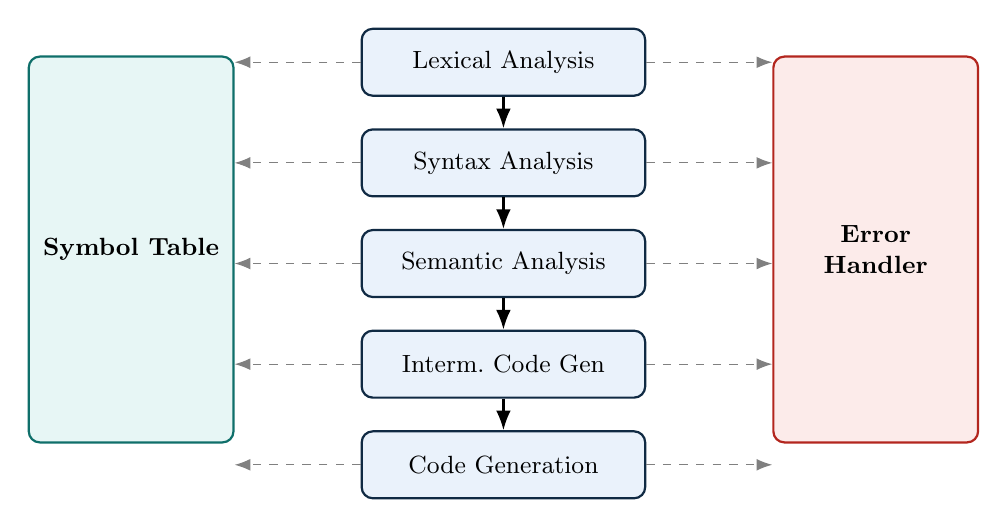
\begin{tikzpicture}[
  ph/.style={draw, thick, rounded corners, minimum height=0.85cm, minimum width=3.6cm, align=center, fill=nuLight, draw=nuNavy, font=\small},
  side/.style={draw, thick, rounded corners, minimum height=4.9cm, minimum width=2.6cm, align=center, font=\small\bfseries, text width=2.3cm},
  node distance=0.4cm
]
  \node[ph] (lex) {Lexical Analysis};
  \node[ph, below=of lex] (syn) {Syntax Analysis};
  \node[ph, below=of syn] (sem) {Semantic Analysis};
  \node[ph, below=of sem] (icg) {Interm.\ Code Gen};
  \node[ph, below=of icg] (cg) {Code Generation};
  \foreach \a/\b in {lex/syn, syn/sem, sem/icg, icg/cg}
    \draw[-{Latex[length=2.5mm]}, thick] (\a) -- (\b);

  \node[side, fill=takeawayTealBg, draw=takeawayTeal, left=1.6cm of syn, yshift=-1.1cm] (st) {Symbol Table};
  \node[side, fill=examRedBg, draw=examRed, right=1.6cm of syn, yshift=-1.1cm] (eh) {Error Handler};

  \foreach \p in {lex, syn, sem, icg, cg}{
    \draw[-{Latex[length=2mm]}, gray, dashed] (\p.west) -- (st.east |- \p.west);
    \draw[-{Latex[length=2mm]}, gray, dashed] (\p.east) -- (eh.west |- \p.east);
  }
\end{tikzpicture}}
\end{center}

\begin{enrichment}[Extra Depth: What Real Symbol Tables Store]
A production compiler's symbol table stores far more than DB's introductory description
suggests: mangled names (for overload resolution in C++/Rust), calling-convention information,
alignment and padding requirements, visibility/linkage (\texttt{static} vs.\ exported), inlining
hints, and --- in languages with generics/templates --- a separate table per instantiation.
Modern compilers often implement it not as one flat table but as a \textbf{chain of nested
scopes} (a scope stack or scope tree), so that entering a block, function, or class pushes a
new scope that shadows outer ones and is popped on exit. LLVM's \texttt{clang} keeps this
information in its \texttt{Decl} hierarchy rather than a single table, reflecting how much richer
real symbol-table designs are compared to the simple table DB introduces.
\end{enrichment}

\section{Grouping the Phases: Front-End, Middle-End, Back-End}

\beyonddb DB's own diagram groups phases into analysis/synthesis, but the vocabulary you will
hear constantly in industry and in later lectures is \textbf{front-end / middle-end / back-end}.
This is not just relabeling --- it reflects a real engineering strategy.

\begin{center}
\renewcommand{\arraystretch}{1.3}
\begin{tabularx}{\textwidth}{@{}l X@{}}
\toprule
\textbf{Group} & \textbf{Contains / Responsibility} \\
\midrule
\textbf{Front-end} & Lexical, syntax, semantic analysis. Language-\emph{specific}: knows the
grammar and type rules of exactly one source language, and lowers it to a common IR. \\
\textbf{Middle-end} & Machine-independent optimization on the IR. Language-\emph{agnostic} and
target-\emph{agnostic}: the same optimization passes (constant folding, dead-code elimination,
inlining) apply no matter which source language or target CPU is involved. \\
\textbf{Back-end} & Code generation and machine-dependent optimization. Target-\emph{specific}:
knows the instruction set, register file, and calling convention of exactly one target
architecture. \\
\bottomrule
\end{tabularx}
\end{center}

\begin{coreidea}[Why This Grouping Is the Whole Point]
If front-ends only ever talk to a shared IR, and back-ends only ever talk to that same shared
IR, then supporting a new \emph{source language} only requires writing one new front-end --- it
automatically gets every optimization and every target the IR already supports. Symmetrically,
supporting a new \emph{target CPU} only requires writing one new back-end --- it automatically
works for every source language already supported. Without this split, you would need to write a
separate optimizer and code generator for every (language, target) \emph{pair} --- the classic
``$M$ languages $\times$ $N$ targets'' problem, needing on the order of $M \times N$ components
instead of $M + N$.
\end{coreidea}

\begin{historynote}
This $M \times N$ argument predates LLVM by decades. In the 1960s, \textbf{T-diagrams}
(popularized by F.\,L.\ Bauer and others) were a standard notation for exactly this problem:
a T-shaped diagram showing a compiler written in language $H$, translating source language $S$
into target language $T$. Compiler writers used T-diagrams to reason about \emph{bootstrapping}
(compiling a new compiler using an existing one) and about how many compilers you actually need
to support $M$ languages on $N$ machines --- precisely the front-end/back-end decoupling
argument above, expressed sixty years earlier with pen-and-paper diagrams instead of shared IR
software.
\end{historynote}

\begin{enrichment}[Extra Depth: The Front/Middle/Back Split in a Real Toolchain --- LLVM]
The clearest concrete instance of this architecture today is LLVM, and it is worth walking
through once here since we will return to it in Lecture 25 for code generation proper.
\begin{itemize}
  \item \textbf{Front-end (Clang, for C/C++/Objective-C):} lexes and parses source into a
  Clang-specific Abstract Syntax Tree (AST), performs semantic analysis and type checking on
  that AST, then \emph{lowers} it into \textbf{LLVM IR} --- a typed, SSA-based (Static Single
  Assignment) intermediate representation that is completely independent of C++ as a language.
  Rust (\texttt{rustc}), Swift, Julia, and Zig all have their own, completely different
  front-ends, but they all emit the \emph{same} LLVM IR.
  \item \textbf{Middle-end (the LLVM optimizer, \texttt{opt}):} a pipeline of dozens of
  independent \textbf{passes} --- e.g.\ \texttt{mem2reg} (promote stack variables to SSA
  registers), \texttt{instcombine} (peephole-simplify instruction sequences),
  \texttt{inline} (function inlining), \texttt{gvn} (global value numbering, subsuming common
  subexpression elimination), \texttt{loop-vectorize} --- each of which reads LLVM IR and
  produces improved LLVM IR. None of these passes know or care whether the original source was
  C++, Rust, or Swift.
  \item \textbf{Back-end (\texttt{llc}, or the integrated code generator):} lowers optimized
  LLVM IR to a specific target's machine code --- x86-64, AArch64, RISC-V, or even WebAssembly,
  selected via a \texttt{-target} triple. Instruction selection, register allocation, and
  instruction scheduling all happen here, specific to that one target.
\end{itemize}
The practical payoff: when Apple Silicon (AArch64) needed a good C++ compiler, no one had to
write a new C++ front-end --- Clang's C++ front-end and every middle-end optimization pass were
already reusable; only a back-end for AArch64 was needed (and it mostly already existed, since
LLVM had supported ARM for years).
\end{enrichment}

\section{The Compiler's Neighbors: Preprocessor, Assembler, Linker \& Loader}

\dbtag The ``compiler'' most people mean when they say \texttt{gcc file.c} is actually a
\textbf{driver program} that invokes several distinct tools in sequence. DB \S2.1--\S2.8 places
the compiler proper in the context of this larger \textbf{language-processing system}.

\begin{center}
\resizebox{\textwidth}{!}{%
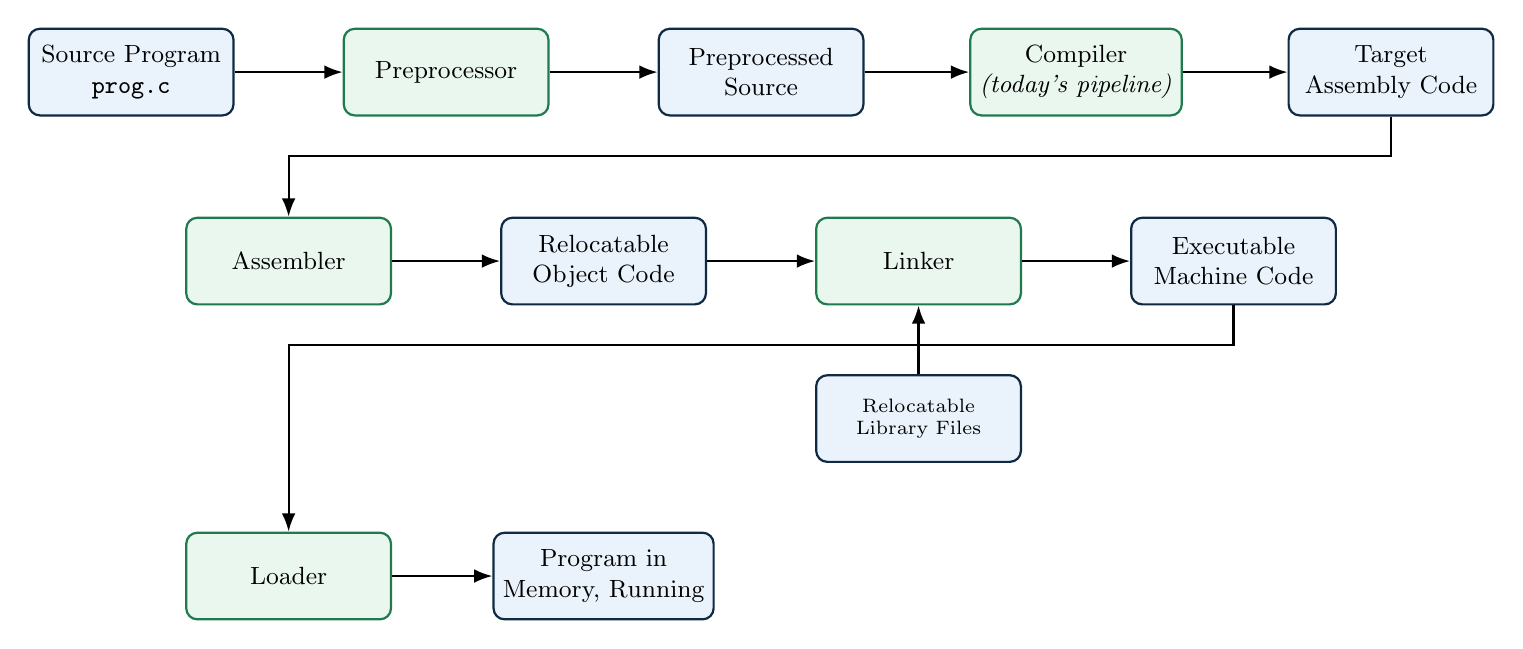
\begin{tikzpicture}[
  box/.style={draw, thick, rounded corners, minimum height=1.1cm, minimum width=2.6cm, align=center, font=\small},
  tool/.style={box, fill=dbGreenBg, draw=dbGreen},
  data/.style={box, fill=nuLight, draw=nuNavy},
  >=Latex
]
  % Row 1: source through target assembly
  \node[data]                       at (0,0)    (src)  {Source Program\\\texttt{prog.c}};
  \node[tool]                       at (4,0)    (cpp)  {Preprocessor};
  \node[data]                       at (8,0)    (isrc) {Preprocessed\\Source};
  \node[tool]                       at (12,0)   (comp) {Compiler\\\emph{(today's pipeline)}};
  \node[data]                       at (16,0)   (asmf) {Target\\Assembly Code};

  % Row 2: assembler through linker
  \node[tool]                       at (2,-2.4) (asm)  {Assembler};
  \node[data]                       at (6,-2.4) (obj)  {Relocatable\\Object Code};
  \node[tool]                       at (10,-2.4)(link) {Linker};
  \node[data]                       at (14,-2.4)(exe)  {Executable\\Machine Code};
  \node[data, font=\small\scriptsize] at (10,-4.4)(lib){Relocatable\\Library Files};

  % Row 3: loader through running program
  \node[tool]                       at (2,-6.4) (load) {Loader};
  \node[data]                       at (6,-6.4) (mem)  {Program in\\Memory, Running};

  \draw[->, thick] (src) -- (cpp);
  \draw[->, thick] (cpp) -- (isrc);
  \draw[->, thick] (isrc) -- (comp);
  \draw[->, thick] (comp) -- (asmf);
  \draw[->, thick] (asmf.south) -- ++(0,-0.5) -| (asm.north);
  \draw[->, thick] (asm) -- (obj);
  \draw[->, thick] (obj) -- (link);
  \draw[->, thick] (lib) -- (link);
  \draw[->, thick] (link) -- (exe);
  \draw[->, thick] (exe.south) -- ++(0,-0.5) -| (load.north);
  \draw[->, thick] (load) -- (mem);
\end{tikzpicture}}
\end{center}

\begin{itemize}
  \item \textbf{Preprocessor.} Handles macro expansion (\texttt{\#define}), file inclusion
  (\texttt{\#include}), and conditional compilation (\texttt{\#ifdef}) \emph{before} the
  compiler proper ever sees the code. It works on raw text, with no notion of the language's
  grammar.
  \item \textbf{Compiler (proper).} Everything in \S1 of this lecture: source $\to$ target
  assembly (or directly to object code, in many modern compilers, skipping a textual assembly
  step).
  \item \textbf{Assembler.} Translates (textual) assembly instructions into \textbf{relocatable
  machine code} --- binary instructions, but with addresses left as symbolic placeholders to be
  filled in later, since the assembler does not yet know the final memory layout.
  \item \textbf{Linker.} Resolves references \emph{between} separately compiled object files and
  libraries --- e.g.\ your \texttt{main.o} calling \texttt{printf}, defined in the C standard
  library, not in your own source. Produces one combined \textbf{executable} with all addresses
  resolved (or marked for the dynamic linker, see below).
  \item \textbf{Loader.} Takes the executable file, allocates memory for it, and places its
  instructions and data into memory so the operating system can begin executing it --- the very
  last step before your program actually runs.
\end{itemize}

\begin{examfocus}
Know precisely which of preprocessor/assembler/linker/loader are considered \emph{part of} ``the
compiler'' in the narrow sense (none of them --- the compiler proper is only the six-phase
pipeline from \S1) versus which are separate programs in the surrounding toolchain that DB
still expects you to know the role of. A common exam trap: ``which phase resolves a call to a
library function like \texttt{printf}?'' --- the answer is the \textbf{linker}, not the compiler.
\end{examfocus}

\begin{enrichment}[Extra Depth: Seeing the Real Pipeline on Your Own Machine]
You can watch this exact pipeline happen with GCC or Clang by stopping it at each stage:
\begin{itemize}
  \item \texttt{gcc -E prog.c -o prog.i} --- run \emph{only} the preprocessor; inspect
  \texttt{prog.i} to see macros expanded and headers inlined.
  \item \texttt{gcc -S prog.i -o prog.s} --- run the compiler proper; \texttt{prog.s} is
  human-readable target assembly.
  \item \texttt{gcc -c prog.s -o prog.o} --- run the assembler; \texttt{prog.o} is a relocatable
  ELF (on Linux) object file. Inspect it with \texttt{objdump -d prog.o} or \texttt{nm prog.o}.
  \item \texttt{gcc prog.o -o prog} --- run the linker, pulling in the C runtime and any
  libraries, producing the final executable.
\end{itemize}
Try this on a one-line \texttt{"hello world"} program: the jump in size and content between
\texttt{prog.i} (hundreds of lines, from expanded standard-library headers) and \texttt{prog.c}
(one line) is a genuinely eye-opening way to internalize what the preprocessor actually does.
\end{enrichment}

\begin{enrichment}[Extra Depth: Static vs.\ Dynamic Linking, and What the Loader Really Does]
DB's loader description is simplified; two refinements matter a great deal in practice:
\begin{itemize}
  \item \textbf{Static linking} copies the code of every library function you use directly into
  your executable at link time. The result is self-contained but larger, and does not benefit
  when the OS wants to share one copy of, say, \texttt{libc}, across many running programs.
  \item \textbf{Dynamic linking} instead records, in the executable, only the \emph{names} of
  needed shared libraries (\texttt{.so} on Linux, \texttt{.dll} on Windows, \texttt{.dylib} on
  macOS). A specialized program, the \textbf{dynamic linker/loader} (\texttt{ld.so} on Linux),
  runs as the executable starts, finds each shared library already resident in memory or maps it
  fresh, and \textbf{patches in} the real addresses of library functions --- a process called
  \textbf{relocation} --- before your \texttt{main} function ever runs. This is why dynamically
  linked executables are smaller on disk but have slightly higher startup latency and a runtime
  dependency on the right library versions being present (colloquially, ``DLL hell'').
  \item \textbf{Position-Independent Code (PIC)} is machine code generated so it can be loaded
  at \emph{any} memory address, not a fixed one --- essential for shared libraries (which may be
  mapped at different addresses in different processes) and for security features like ASLR
  (Address Space Layout Randomization). Generating PIC is a back-end code-generation decision,
  another example of how deep the ``compiler'' choices reach into topics normally considered OS
  territory.
\end{itemize}
\end{enrichment}

\begin{enrichment}[Extra Depth: Build Systems Are Compiler Orchestration at Scale]
Everything above describes compiling \emph{one} file. Real projects have thousands. The tools
that decide \emph{which} files need recompiling and in what order are themselves built on the
phase model above:
\begin{itemize}
  \item \textbf{Make / Ninja} track file modification timestamps and a dependency graph to
  avoid recompiling unchanged files --- essentially caching the output of the ``compiler'' node
  in the pipeline diagram above, keyed by source-file identity and timestamp.
  \item \textbf{ccache / sccache} go further: they hash the \emph{preprocessed} source
  (post-preprocessor, pre-compiler) plus compiler flags, and cache the resulting object file, so
  an unchanged file compiled with unchanged flags never re-invokes the compiler proper at all ---
  directly exploiting the preprocessor/compiler boundary from \S4.
  \item \textbf{Bazel and other hermetic build systems} extend caching across an entire team or
  CI fleet: if any engineer, anywhere, has already built a given (source, flags, toolchain)
  combination, everyone else can fetch the cached object/executable instead of recompiling.
  \item \textbf{Link-Time Optimization (LTO / ThinLTO)} deliberately \emph{breaks} the strict
  separate-compilation model: instead of each \texttt{.c} file being optimized in isolation
  before linking, LTO defers whole-program optimization to link time, when the optimizer can see
  every translation unit at once and, e.g., inline a function across what used to be file
  boundaries. This directly trades the modularity of the pipeline in \S4 for better runtime
  performance.
\end{itemize}
\end{enrichment}

\begin{enrichment}[Extra Depth: The Front-End's Second Career --- IDEs and Language Servers]
The front-end (lexer + parser + semantic analyzer) is valuable even when no target code is ever
generated. This observation underlies the \textbf{Language Server Protocol (LSP)}: an editor
like VS Code or Neovim talks to a background process (a ``language server'') that re-runs a
language's front-end on every keystroke to provide autocomplete, jump-to-definition, and
real-time error squiggles --- all without ever reaching code generation. \texttt{clangd} (built
directly on Clang's front-end), \texttt{rust-analyzer}, and \texttt{gopls} are all, in effect,
``compilers with the back end removed and an editor bolted on instead.'' This is a direct,
practical payoff of the front-end/back-end separation from \S3: a front-end built for compilation
can be repurposed wholesale for tooling.
\end{enrichment}

\section{Self-Check Questions}

\begin{enrichment}[Practice -- Not Graded]
\begin{enumerate}
  \item Place the following in correct pipeline order: semantic analysis, linking, assembly,
  lexical analysis, loading, syntax analysis, preprocessing, code generation.
  \item A program calls a function defined in a library it never \texttt{\#include}s a
  declaration for, but the linker still resolves the call successfully because the symbol name
  matches at link time. Which phase would have caught this as an error if the declaration truly
  were missing, and why didn't it?
  \item Explain, in the M-languages/N-targets argument, why a shared IR turns an
  $M \times N$ problem into an $M + N$ problem. What is the "shared IR" in LLVM's case?
  \item Why does dynamic linking trade smaller executables for slower startup, while static
  linking does the opposite?
  \item \texttt{clangd} never performs code generation. Which phases of the pipeline does it
  still need to run, and why are those enough to power features like ``jump to definition''?
\end{enumerate}
\end{enrichment}

\begin{takeaways}
\begin{itemize}
  \item A compiler's six classical phases, in order: lexical analysis, syntax analysis, semantic
  analysis, intermediate code generation, code optimization, code generation.
  \item These split into an \textbf{analysis} half (front end: builds an IR and symbol table)
  and a \textbf{synthesis} half (back end: builds the target program from that IR).
  \item The \textbf{symbol table} and \textbf{error handler} are not phases in the pipeline ---
  they run alongside every phase.
  \item The \textbf{front-end/middle-end/back-end} split (language-specific $\to$
  language-and-target-agnostic $\to$ target-specific) is what lets one shared IR (like LLVM IR)
  turn an $M \times N$ language/target problem into an $M + N$ problem.
  \item The compiler proper sits inside a larger toolchain: \textbf{preprocessor} (before) and
  \textbf{assembler, linker, loader} (after) are separate programs, not phases of the compiler
  itself, though DB expects you to know each one's job.
  \item Front-ends have value beyond compilation: build caching, LTO, and language servers
  (\texttt{clangd}, \texttt{rust-analyzer}) all repurpose pieces of this pipeline for other ends.
\end{itemize}
\end{takeaways}

\section*{References for This Lecture}
\begin{itemize}
  \item [DB] Aho, Lam, Sethi, Ullman. \textit{Compilers: Principles, Techniques, and Tools}, 2nd ed., \S1.2, \S2.1--\S2.8.
  \item [PP] Scott. \textit{Programming Language Pragmatics}, \S1.5, \S1.6.
\end{itemize}

\end{document}
